\documentclass[14pt, a4paper]{article}
\usepackage{minitoc}
\usepackage[left=3.00cm, right=2.5cm, top=2.00cm, bottom=2.00cm]{geometry}
\usepackage{amsmath}
\usepackage{amssymb}
\usepackage{amsthm}
\usepackage{mathtools}
\usepackage{graphicx}
\usepackage{algpseudocode}
\usepackage{algorithm}
\usepackage{blindtext}
\usepackage{setspace}
\usepackage[utf8]{inputenc}
\usepackage[utf8]{vietnam}
\usepackage[center]{caption}
\usepackage[shortlabels]{enumitem}
\usepackage{fancyhdr} % header, footer
\usepackage{hyperref} % loại bỏ border với mục lục và công thức
\usepackage[nonumberlist, nopostdot, nogroupskip]{glossaries}
\usepackage{glossary-superragged}
\setglossarystyle{superraggedheaderborder}
\pagestyle{fancy}
%\usepackage[style=numeric,sortcites]{biblatex}
%\addbibresource{ref.bib}
%\usepackage[numbers]{natbib}
\usepackage{indentfirst}
\usepackage[natbib,backend=biber,style=ieee, sorting=ynt]{biblatex}
\bibliography{ref.bib}

\graphicspath{{./figures/}}

\makenoidxglossaries

% Danh mục thuật ngữ

\newglossaryentry{RNN}
{
	name={RNN},
	description={Recurrent Neural Network}
}

\newglossaryentry{LSTM}
{
	name={LSTM},
	description={Long Short Term Memory}
}

\newglossaryentry{GRU}
{
	name={GRU},
	description={Gated Recurrent Unit}
}

\newglossaryentry{BERT}
{
	name={BERT},
	description={Bidirectional Encoder Representations from Transformer}
}

\newglossaryentry{BLEU}
{
	name={BLEU},
	description={Bilingual Language Evaluation Understudy}
}

\newglossaryentry{CNN}
{
	name={CNN},
	description={Convolutional Neural Networks}
}

\hypersetup{
    colorlinks=false,
    pdfborder={0 0 0},
}

\title{Báo cáo bài tập lớn môn học}

\author{Nguyễn Chí Thanh}


\fancyhf{}
\rhead{\textbf{Phát triển phần mềm nâng cao cho tính toán khoa học}}
\lhead{\textbf{GVHD: TS. Vũ Tiến Dũng}}
\rfoot{\thepage}
\lfoot{\textbf{Ứng dụng Deep Learning xây dựng phần mềm tự động sinh mô tả ảnh}}
\renewcommand{\headrulewidth}{0.4pt}
\renewcommand{\footrulewidth}{0.4pt}

\numberwithin{equation}{section}
\numberwithin{algorithm}{section}
\numberwithin{figure}{section}

\setlength{\parindent}{0.5cm}

\setcounter{secnumdepth}{3} % Cho phép subsubsection trong report
\setcounter{tocdepth}{3} % Chèn subsubsection vào bảng mục lục

\newtheorem{dl}{Định lý}
\newtheorem{md}{Mệnh đề}
\newtheorem{bd}{Bổ đề}
\newtheorem{dn}{Định nghĩa}
\newtheorem{hq}{Hệ quả}

\numberwithin{dl}{section}
\numberwithin{md}{section}
\numberwithin{bd}{section}
\numberwithin{dn}{section}
\numberwithin{hq}{section}

\doublespacing

\begin{document}
    \cleardoublepage
    \pagenumbering{gobble}
    \tableofcontents
    \newpage
    \listoffigures
    \newpage
    \glsaddall 
    \renewcommand*{\glossaryname}{Danh mục từ viết tắt}
    %\renewcommand*{\glossaryname}{Danh mục thuật ngữ}
    %\renewcommand*{\acronymname}{Danh sách từ viết tắt}
    %\renewcommand*{\entryname}{Viết tắt}
    %\renewcommand*{\descriptionname}{Viết đầy đủ}
    \printnoidxglossary
    \cleardoublepage
    \pagenumbering{arabic}

    %\maketitle

    \newpage

    \nocite{*}

    \begin{center}
    \section*{LỜI MỞ ĐẦU}
    \end{center}
    \addcontentsline{toc}{section}{{\bf LỜI MỞ ĐẦU}\rm}

    \newpage

    \section{Tổng quan về bài toán sinh mô tả ảnh}

    \subsection{Bài toán dịch máy (\textit{Machine Translation})} \label{Machine-Translation}
    Bài toán sinh mô tả ảnh là một bài toán rất thường gặp trong các ứng dụng của Deep Learning.
    Do đầu ra của bài toán sinh mô tả ảnh là ngôn ngữ, nên có thể xem mô hình sinh mô tả ảnh thuộc lớp mô hình xử lý ngôn ngữ tự nhiên.
    Vì vậy, kiến trúc của mô hình sinh mô tả ảnh kế thừa chủ yếu từ bài toán dịch máy (\textit{Machine Translation}).
    
    Bài toán dịch máy là việc dịch tự động một đoạn văn bản từ ngôn ngữ này sang ngôn ngữ khác.
    Giải quyết bài toán với các mạng neuron được gọi là dịch máy neuron (\textit{Neural Machine Translation}).
    Dịch máy có ứng dụng rất lớn trong đời sống xã hội cũng như phục vụ công tác nghiên cứu khoa học. 
    Một phần mềm nổi bật nhất về bài toán dịch máy rất phổ biến hiện nay là Google dịch (\textit{Google Translate}).
    
    Dịch máy là một bài toán rất được quan tâm bởi cộng đồng xử lý ngôn ngữ tự nhiên (\textit{Natural Language Processing}) đặc biệt là dịch máy neuron đã đạt được rất nhiều bước tiến trong những năm vừa qua.
    Cấu trúc của một mô hình dịch máy neuron điển hình gồm hai thành phần chính:

    \begin{itemize}
        \item Thành phần mã hóa (\textit{Encoder}): Thành phần này có nhiệm vụ mã hóa câu đầu vào thuộc ngôn ngữ nguồn thành một vector. Vector này trở thành đầu vào hoặc được biến đổi trở thành trạng thái đầu của thành phần tiếp theo.
        \item Thành phần giải mã (\textit{Decoder}): Thành phần này nhận vector đầu ra từ thành phần encoder, biến đổi vector này thành đầu vào hoặc trạng thái đầu của thành phần này. Đầu ra của thành phần này là các từ trong ngôn ngữ đích. Quá trình đưa ra từng từ trong ngôn ngữ đích được gọi là quá trình dịch.
    \end{itemize}

    \begin{figure}[h!] \centering

        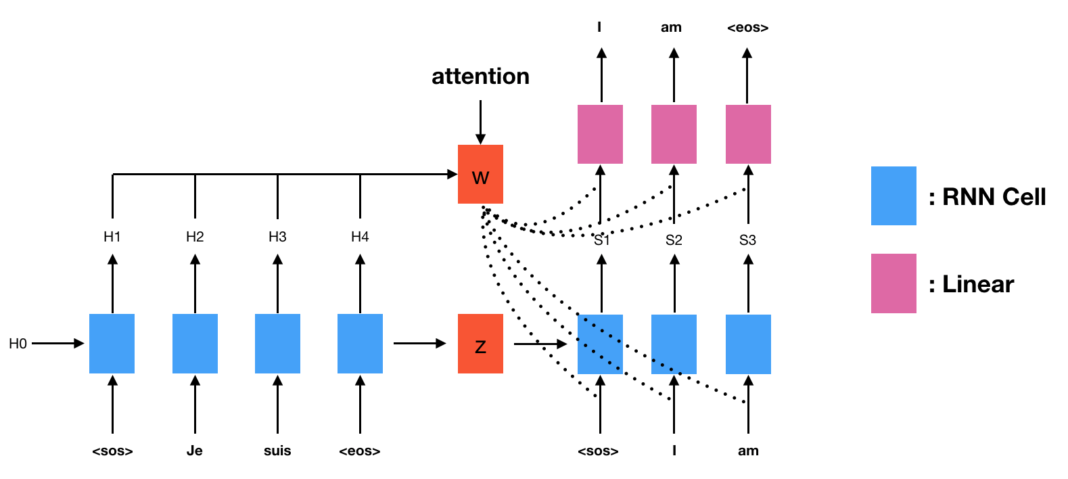
\includegraphics[scale=0.35]{Neural_Machine_Translation_Architecture.png}
        \caption{Cấu trúc chung của một mô hình dịch máy neuron.}
    
        \label{fig:Neural_Machine_Translation_Architecture}
    \end{figure}

    Một cấu trúc điển hình của một mô hình dịch máy neuron được minh họa ở hình \ref{fig:Neural_Machine_Translation_Architecture}.
    Ngoài hai thành phần quan trọng kể trên, còn có một thành phần quan trọng khác không bắt buộc nhưng rất hay xuất hiện ở trong các mô hình dịch máy là thành phần sử dụng cơ chế tập trung (\textit{Attention}).
    Một số công trình mà mô hình đóng một vai trò quan trọng: \cite{bahdanau2014neural}, \cite{luong2014addressing}, \cite{jean2014using}, \cite{luong2015effective}, \cite{tang2016neural}, \cite{wang2016memory}, \cite{li2016towards}, \cite{tu2016modeling}, \cite{shen2015minimum}, \cite{zhou2016deep}.

    Cơ chế Attention bản chất chính là sự chú ý. Trong quá trình dịch, mô hình sẽ cần tập trung vào từ nào ở trong câu đầu vào để đưa ra lựa chọn từ nào ở trong ngôn ngữ đích.
    Lý do cơ chế Attention ra đời là vì mô hình chỉ có hai thành phần encoder và decoder có một hạn chế rất lớn. Encoder sẽ phải nén toàn bộ thông tin của câu đầu vào thành một vector, rõ ràng đây không phải là điều hợp lý.
    Đặc biệt khi câu đầu vào dài thì enocder phải đưa toàn bộ các thông tin vào một vector thì nó sẽ phải làm mất hoặc quên một thông tin nào đó.
    Mặt khác, thành phần decoder chỉ thấy một vector biểu diễn đầu vào duy nhất, dù mỗi bước thời gian (\textit{timestep}) khác nhau thì các thành phần khác nhau của câu đầu vào có ích hơn phần khác.
    Nhưng nếu chỉ có một vector duy nhất, việc để chọn ra thông tin hợp lý tại mỗi timestep gần như không khả thi.

    Hai cơ chế Attention hay được sử dụng phổ biến nhất là Bahdanau Attention \cite{bahdanau2014neural} và Luong Attention \cite{luong2014addressing}. Trong bài tập lớn, nhóm sẽ chỉ sử dụng và trình bày Bahdanau Attention.
    Ta giả sử có một câu đầu vào $\bold{X}$ với độ dài là $L$ từ, và một câu dịch tương ứng $\bold{Y}$ với độ dài $C$ từ:

    \begin{equation}
        \begin{aligned}
            \bold{X} = \lbrack \bold{x}_1, \bold{x}_2, \dots, \bold{x}_L \rbrack, \bold{x}_i \in \mathbb{R}^D \\
            \bold{Y} = \lbrack \bold{y}_1, \bold{y}_2, \dots, \bold{y}_C \rbrack, \bold{y}_t in \mathbb{R}^K
        \end{aligned}
    \end{equation}

    Một từ trong một timestep $t$ của thành phần đầu ra của decoder phụ thuộc vào đầu ra timestep phía trước $\bold{y}_{t-1}$, trạng thái ẩn của decoder $\lbrace \bold{c}_t, \bold{h}_t \rbrace$ và vector bối cảnh $\bold{z}_t$ được tính theo công thức tổng quát:

    \begin{equation}
        p(\bold{y}_t \vert \lbrace \bold{y}_1, \bold{y}_2, \dots, \bold{y}_{t-1} \rbrace, \bold{X}) = g(\bold{y}_{t-1}, \lbrace \bold{c}_t, \bold{h}_t \rbrace, \bold{z}_t)
    \end{equation}

    Trạng thái ẩn $\lbrace \bold{c}_t, \bold{h}_t \rbrace$ của decoder được tính một mạng RNN với thông tin từ trạng thái ẩn của timestep trước, đầu ra của bước trước và vector bối cảnh:
    
    \begin{equation}
        \lbrace \bold{c}_t, \bold{h}_t \rbrace = f(\bold{y}_{t-1}, \lbrace \bold{c}_{t-1}, \bold{h}_{t-1} \rbrace, \bold{z}_t) \forall t=1,\dots,C
    \end{equation}

    Vector bối cảnh là vector được tính bằng tổng trọng số của đầu ra của encoder tại đầu thứ $i$, $\alpha_{ti}$ biểu thị trọng số mức độ chú ý với đầu ra $\bold{a}_i$ ở timestep thứ $t$:

    \begin{equation}
        \bold{z}_t = \sum_{i=1}^{L}\alpha_{ti}\bold{a}_i
    \end{equation}

    Với $\alpha_{ti}$ thực chất được tính từ hàm softmax là trọng số riêng được tính từ đầu ra thứ $i$ của encoder. Hàm softmax là một cách để chuẩn hóa các $\alpha_{ti}$ cho $\sum_{i=1}^{L}\alpha_{ti}=1$

    \begin{equation}
        \alpha_{ti} = \dfrac{e_{ti}}{\sum_{k=1}^{L} e_{tk}}
    \end{equation}

    $e_{ti}$ là tương quan giữa đầu ra $\bold{y}_t$ bước thứ $t$ và đầu vào $\bold{x}_i$ bước thứ $i$ thường được tính bằng một mạng neuron:

    \begin{equation}
        e_{ti} = f_{\text{att}}(\lbrace \bold{c}_{t-1}, \bold{h}_{t-1} \rbrace, \bold{a}_i)
    \end{equation}

    Trong \cite{bahdanau2014neural}, tác giả đề xuất một Attention model với công thức:

    \begin{equation}
        e_{ti} = f_{\text{att}}(\lbrace \bold{c}_{t-1}, \bold{h}_{t-1} \rbrace, \bold{a}_i) = \bold{v}_{\bold{a}}^T \tanh (\bold{W} \lbrace \bold{c}_{t-1}, \bold{h}_{t-1} \rbrace + \bold{U}\bold{a}_i)
    \end{equation}

    với $\bold{W} \in \mathbb{R}^{2D \times D}$ và $\bold{U}^{D \times D}$, $\bold{v}_{\bold{a}} \in \mathbb{R}^{D}$ là các ma trận trọng số được huấn luyên.

    Thực chất cơ chế Attention giúp cho mô hình tập trung vào các phần quan trọng của dữ liệu, bằng việc tạo một mạng neuron đơn giản tính các trọng số $\alpha_{ti}$ để đánh lại các trọng số của các đầu ra của encoder $\bold{a}_i$.
    Trong mô hình dịch máy neuron, việc này giúp mô hình tập trung hơn vào những từ quan trọng trong câu đầu vào $\bold{X}$, từ đó dự đoán ra từ $\bold{y}_t$ tiếp theo tại decoder, được biểu diễn bằng các ô sáng màu trong Attention map ở hình \ref{fig:Attention_Map}

    \begin{figure}[h!] \centering

        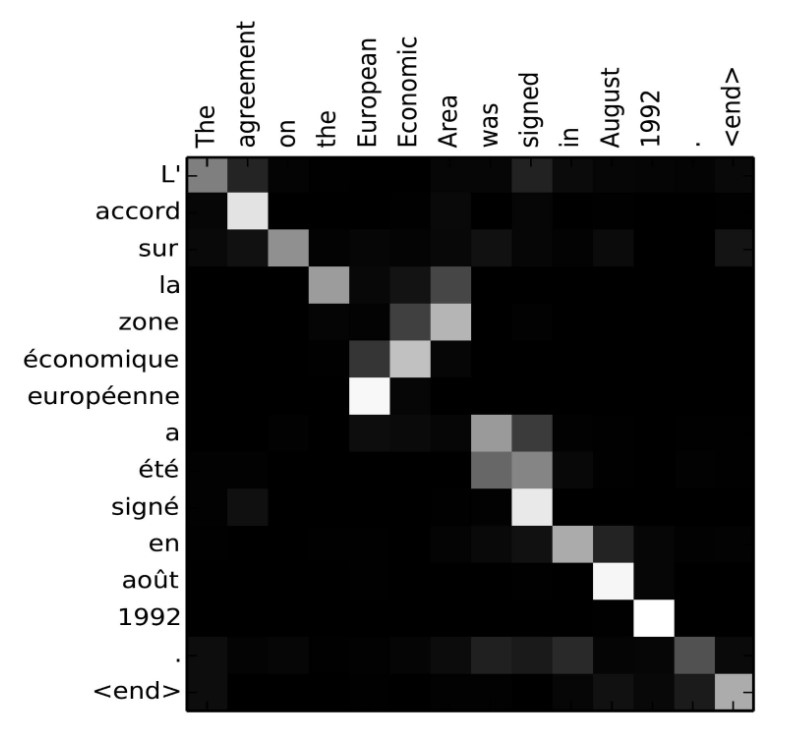
\includegraphics[scale=0.5]{Attention_Map.jpg}
        \caption{Ma trận biểu diễn mức độ tương quan giữa từng từ ở câu đầu vào (tiếng Pháp) và câu được dịch đầu ra (tiếng Anh).}
    
        \label{fig:Attention_Map}
    \end{figure}

    Một số cơ chế tính Attention khác:

    \begin{itemize}
        \item Content-base Attention: $e_{ti}=\cos(\lbrace \bold{c}_{t-1}, \bold{h}_{t-1} \rbrace, \bold{a}_i)$ được đề xuất trong \cite{graves2014neural}
        \item Additive Attention chính là cơ chế Attention được trình bày ở trên \cite{bahdanau2014neural}
        \item Dot-Product Attention được đề xuất trong \cite{luong2015effective}
        \item General Attention được đề xuất trong \cite{luong2015effective}
    \end{itemize}

    Ngoài ra còn một số các loại cơ chế Attention khác:

    \begin{itemize}
        \item Self-Attention.
        \item Soft/Hard Attention.
        \item Global/Local Attention.
    \end{itemize}

    \textbf{Self-Attention:} là một cơ chế Attention chỉ dùng cho một câu. 
    Ta sẽ tự tạo một ma trận tương quan giữa từng từ trong câu để hiểu những phần nào của câu sẽ liên quan đến nhau.
    Cơ chế này đã chứng minh được sự hiệu quả trong các bài toán xử lý ngôn ngữ tự nhiên như tóm tắt văn bản, dịch máy,... 
    Cùng với self-attention là sự ra đời của cấu trúc Transformer \cite{vaswani2017attention} cho phép thay thế hoàn toàn kiến trúc mạng neuron RNN bằng các mô hình kết nối đầy đủ (\textit{fully connected}) mà vẫn cho kết quả tốt.


    \textbf{Soft/Hard Attention:} Hai cơ chế này được áp dụng cho bài toán sinh mô tả ảnh.
    Ảnh đầu tiên sẽ được trích xuất đặc trưng qua mạng neuron tích chập CNN (\textit{Convolutional Neural Networks}) sau đó mạng LSTM kết hợp với cơ chế Attention sẽ thực hiện nhiệm vụ giải mã (\textit{decoding}) các đặc trưng để tạo ra mô tả cho ảnh.
    Hai cơ chế Soft Attention và Hard Attention được phân biệt như sau:

    \begin{itemize}
        \item \textbf{Soft Attention:} sử dụng các trọng số $\alpha_{ti}$ để tính ra vector bối cảnh và nó là hàm khả vi nên có thể sử dụng giảm theo gradient (\textit{Gradient Descent}) và lan truyền ngược (\textit{Back Propagation}) để huấn luyện. 
        Tuy nhiên do tính trên toàn bộ đầu vào thì đối với các bài toán liên quan đến ảnh thì chi phí tính toán sẽ rất cao khi kích thước ảnh lớn.
        \item \textbf{Hard Attention:} thay vì tính trung bình có trọng số của tất cả các vector đầu ra của encoder thì sử dụng điểm Attention để lựa chọn vị trí của vector thích hợp nhất.
        Hard Attention thường được huấn luyện bằng các phương pháp học tăng cường (\textit{Reinforcement Learning}). Ưu điểm của cơ chế này là chi phí tính toán thấp hơn, nhưng yêu cầu kỹ thuật phức tạp để huấn luyện.
    \end{itemize}

    \textbf{Global/Local Attention:} Các mô hình mặc định hay dùng cơ chế Global Attention là cơ chế Attention sẽ tính toán dựa trên toàn bộ đầu vào.
    Nhưng các bài toán đôi khi có thể có chi phí tính toán tốn kém hoặc không cần thiết. Do vậy một số mô hình đưa ra cơ chế Local Attention, chỉ quan tâm đến một phần của đầu vào.
    Local Attention có thể coi giống như Hard Attention. Ngoài ra có thể so sánh Global Attention như một mạng fully connected, còn Local Attention thì giống như mạng neuron tích chập CNN.
    Hình \ref{fig:Local_Global_Attention} so sánh sự khác biệt giữa hai cơ chế Attention.

    \begin{figure}[h!] \centering

        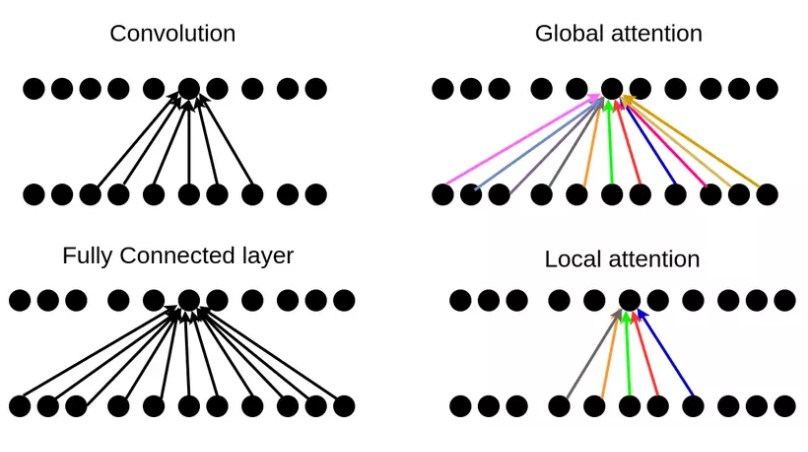
\includegraphics[scale=0.4]{Local_Global_Attention.jpg}
        \caption{So sánh hai cơ chế Global Attention và Local Attention}
    
        \label{fig:Local_Global_Attention}
    \end{figure}

    \subsection{Bài toán sinh mô tả ảnh}

    Ở mục \ref{Machine-Translation} ta đã giới thiệu tổng quan về cấu trúc của một mô hình dịch máy và cơ chế Attention. 
    Ở mục này ta sẽ giới thiệu cấu trúc của một mô hình sinh mô tả ảnh. Cấu trúc của một mô hình sinh mô 

    \newpage
    \addcontentsline{toc}{section}{TÀI LIỆU THAM KHẢO}
    %\bibliographystyle{IEEEtraN}
    %\bibliography{ref}
    %\pagestyle{plain}
    \printbibliography[title={TÀI LIỆU THAM KHẢO}]

    %\newpage
    %\printbibliography
\end{document}